% This must be in the first 5 lines to tell arXiv to use pdfLaTeX, which is strongly recommended.
\pdfoutput=1
% In particular, the hyperref package requires pdfLaTeX in order to break URLs across lines.

\documentclass[11pt]{article}

% Remove the "review" option to generate the final version.
\usepackage[review]{EMNLP2023}

% Standard package includes
\usepackage{times}
\usepackage{latexsym}

% New packages
\usepackage{lipsum}
\usepackage{booktabs}
\usepackage{mystyle}
\usepackage{multirow}

% For proper rendering and hyphenation of words containing Latin characters (including in bib files)
\usepackage[T1]{fontenc}
% For Vietnamese characters
% \usepackage[T5]{fontenc}
% See https://www.latex-project.org/help/documentation/encguide.pdf for other character sets

% This assumes your files are encoded as UTF8
\usepackage[utf8]{inputenc}

% This is not strictly necessary, and may be commented out.
% However, it will improve the layout of the manuscript,
% and will typically save some space.
\usepackage{microtype}

% This is also not strictly necessary, and may be commented out.
% However, it will improve the aesthetics of text in
% the typewriter font.
\usepackage{inconsolata}


\newcommand{\justin}[1]{{{\textcolor{purple}{(Justin: #1)}}}}
\newcommand{\derek}[1]{{{\textcolor{blue}{(Derek: #1)}}}}
\newcommand{\wenting}[1]{{{\textcolor{orange}{(Wenting: #1)}}}}
\newcommand{\daniel}[1]{{{\textcolor{red}{(Daniel: #1)}}}}
\newcommand{\srush}[1]{{{\textcolor{green}{(Sasha: #1)}}}}


% If the title and author information does not fit in the area allocated, uncomment the following
%
%\setlength\titlebox{<dim>}
%
% and set <dim> to something 5cm or larger.

\title{Tool-based Language Models for Grounded Dialogue}

% Author information can be set in various styles:
% For several authors from the same institution:
% \author{Author 1 \and ... \and Author n \\
%         Address line \\ ... \\ Address line}
% if the names do not fit well on one line use
%         Author 1 \\ {\bf Author 2} \\ ... \\ {\bf Author n} \\
% For authors from different institutions:
% \author{Author 1 \\ Address line \\  ... \\ Address line
%         \And  ... \And
%         Author n \\ Address line \\ ... \\ Address line}
% To start a seperate ``row'' of authors use \AND, as in
% \author{Author 1 \\ Address line \\  ... \\ Address line
%         \AND
%         Author 2 \\ Address line \\ ... \\ Address line \And
%         Author 3 \\ Address line \\ ... \\ Address line}

\author{
Justin T. Chiu  \\
Cornell Tech \\
\texttt{jtc257@cornell.edu}
\And
Wenting Zhao \\
Cornell University \\
\texttt{wz346@cornell.edu}
\And
Derek Chen \\
Startup \\
\texttt{derek@startup.com}
\And
Alexander M. Rush \\
Cornell Tech \\
\texttt{arush@cornell.edu}
\And
Daniel Fried \\
Carnegie Mellon University \\
\texttt{dfried@cs.cmu.edu} 
}

\begin{document}
\maketitle
\begin{abstract}
%Two main points:
%1. Low-resource / minimal supervision.
%2. Code for step-by-step reasoning.

%Large language models, when given access to tools such as a code interpreters and computer vision models,
%are able to perform grounded reasoning with minimal supervision.
%Prior work has tested tool-based language models in non-interactive settings.
We study the use of tool-based language models in grounded dialogue.
Out-of-domain generalization is particularly challenging in grounded dialogue,
where language models may easily be exposed to unexpected forms of grounding.
We build a modular dialogue system that allows language models to do what they do best:
understand language, while deferring other tasks, such as grounding and dialogue state tracking,
to more suitable components.
Our system uses language models to generate code in response to partner utterances,
a symbolic planner to decide what to say next,
and a rule-based templated generator to realize symbolic plans into text.
The generated code is used to both manipulate dialogue state, represented as code, as well as perform grounding.
We evaluate our system on a challenging dialogue task, \textsc{OneCommon},
where partners ground discussion on abstract images of scattered dots.
Humans attain a success rate of 65.8\% in the most challenging setting of \textsc{OneCommon}.
Our system achieves strong results in language understanding,
selfplay, and human play.
\end{abstract}


\section{Introduction}
Topic sentence: Large language models have shortcomings, in particular grounding.
Recent work has shown that tool use can adapt ungrounded language models
to grounded tasks with minimal supervision.
Describe code as policies, vipergpt, chatgpt plugins,
which bake in task-specific biases.

Topic sentence: Tool-use has mostly been demonstrated in the single-turn setting,
other than the commercial success of ChatGPT.
The challenge of grounded dialogue is dialogue state tracking and reasoning while
grounding conversation.

Topic sentence: We explore ways methods for applying LLMs to solving grounded tasks.
Method overview: read, plan, write.
Cast reading as code generation.

Topic sentence: We focus on \textsc{OneCommon}, a challenging grounded dialogue task.
Description of what's hard about \textsc{OneCommon}.
Also argue that in dialogue, data collection might be even harder.
Results.

\begin{figure}[t]
\setlength{\abovecaptionskip}{0pt}
grounding

\centering

\scalebox{1.1}{
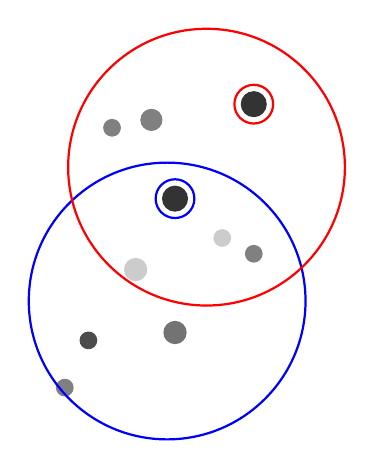
\begin{tikzpicture}

%\filldraw[gray!40] (0,0) circle (.3em);
%\filldraw[gray!100] (.25,0) circle (.38em);
%\filldraw[gray!160] (.5,0) circle (.45em);

\filldraw[gray!160] (-.2,.6) circle (.45em); % 766
\filldraw[gray!40] (-.7,-.3) circle (.4em); % 51
\filldraw[gray!40] (.4,.1) circle (.3em); % 52
\filldraw[gray!100] (.8,-.1) circle (.3em); % 66

% left
\filldraw[gray!140] (-1.3,-1.2) circle (.3em); % 13
\filldraw[gray!100] (-1.6,-1.8) circle (.3em); % 14
\filldraw[gray!110] (-.2,-1.1) circle (.4em); % 74

% right
\filldraw[gray!100] (-1,1.5) circle (.3em); % 28
\filldraw[gray!100] (-.5,1.6) circle (.38em); % 69
\filldraw[gray!160] (.8,1.8) circle (.45em); % 26

% left selects 76
\draw[blue,thick] (-.2,.6) circle (.7em);
% right selects 26
\draw[red,thick] (.8,1.8) circle (.7em);

\draw[blue,thick] (-.3,-.7) circle (5em);
\draw[red,thick] (.2,1) circle (5em);
\end{tikzpicture}
}

\vspace{1em}

\small
\begin{tabular}[b]{@{}l@{}l@{}}
\toprule
{\color{blue} A}:\;&I have one large black dot by itself. Do you have it? \\
{\color{red} P}:\;&Yes, I do have that. \\
{\color{blue} A}:\;&Let's pick that one. \\
{\color{red} P}:\;&<select> {\color{red} red} \\
{\color{blue} A}:\;&<select> {\color{blue} blue}\\
\bottomrule
\end{tabular}

\vspace{1em}

\caption{
An example of perspective-dependent ambiguity from a dialogue {\color{blue}agent} and human {\color{red}partner} playing \textsc{OneCommon}, taken from the evaluation of \citet{fried}.
The players have different but overlapping circular views of a shared board,
which contains dots of different shades, shapes, and sizes.
The agent and partner must collaborate through dialogue in order to find and
select a shared dot.
This dialogue ends in failure, as the agent and partner did not account for perspective-ambiguity and prematurely selected different dots.
}
\label{fig:oc}
\end{figure}


\section{Related work}

\paragraph{Tool-based language models}
Code-as-policies, ViperGPT, PAL, toolformer, VisProg.
Difference: 

\paragraph{Conversational tool-based language models}
VisualChatGPT, chatgpt with plugins.
Difference:

\paragraph{Executable dialogue state tracking}
SMCalFlow.
Difference:

\paragraph{Task-oriented dialogue}
Task-oriented dialogue often uses multi-turn model-based planning.
Here planning is performed in the space of language via rollouts or tree-search
\citep{dnd,yarats2017rollout,ingress,jang2020bapomdp}.
%Our work reduces perspective-dependent ambiguity by incorporating a distribution over unobserved context into the partner model.
While we use a single-turn planning heuristic,
our focus on improving partner models is complementary to multi-turn planning and can be combined in future work.


\section{Grounded dialogue with tool-based language models}
We decompose dialogue into a sequence of three steps: reading, planning, and writing.

\subsection{Reading}
Language to python translation with execution.

\subsection{Planning}
Ask a new question, a follow-up question, or select.

\subsection{Writing}
Realize the plan into language.

\section{Experimental setup}
\label{sec:exp}
We evaluate our method, the Partner Planner, on the \textsc{OneCommon} dataset \citep{onecommon}.
We perform two evaluations:
First, we evaluate the number of incorrectly resolved plans generated by the Partner Planner given a static, natural language dataset.
Second, we evaluate the Partner Planner in dynamic, symbolic selfplay.


\textbf{Static plan evaluation}
In order to show that resolving perspective-dependent
ambiguity reduces errors,
we perform automatic evaluation of plans by evaluating whether the agent plan is incorrectly resolved by the partner model.
A plan is incorrectly resolved if the plan is not empty and the partner does not resolve the plan to any
of the agent's intended referents.
We evaluate this without language by directly feeding the feature
representation of plans from the agent to the partner, who is a Partner Planner.

We generate plans given natural language dialogue history from a validation split of \textsc{OneCommon} following prior work \citep{fried}.\footnote{
Prior work used 10-fold cross-validation.
We use models from prior work trained on one fold, and evaluate our approach
on the validation set for that fold.
In particular, we use fold 1 from prior work.
}
For each turn in the human-generated dialogue, we generate a plan from our model
and label that plan as either a success or failure using the procedure above.
We evaluate on 518 validation games, which have different numbers of shared dots: either 4, 5, or 6.
Fewer shared dots results in more perspective-dependent ambiguity.

\textbf{Symbolic selfplay}
We also evaluate the Partner Planner on symbolic selfplay,
where it plays the full \textsc{OneCommon} game with a copy of itself using symbolic communication.
We evaluate only on the setting with the most perspective-dependent ambiguity, 4 shared dots.
In symbolic selfplay, agents must perform planning, belief updates, and selection.
The Partner Planner is able to exactly communicate confirmations and dot features (bucketed size, color, and relative positions).
We compare the game success rate of the Partner Planner to success rate of the baseline by \cite{fried} and human performance on language selfplay.
Language inherently has more noise than symbolic representations,
meaning symbolic selfplay is an upper bound on performance with language.

\textbf{Systems}
We focus evaluation on the Partner Planner,
which reasons about shared and unshared dots.
We consider an ablated version, which does not model unshared dots.

As a baseline, we compare to an agent from prior work, which does not account for
perspective-dependent ambiguity \citep{fried}.
The baseline model chooses plans based on the round-trip probability from an utterance back to the plan,
which is an egocentric heuristic and also does not account for
uncertainty over shared dots.
The baseline agent chooses 8 plans and 64 utterances for each plan, then chooses the
plan and utterance pair with the highest probability of recovering the plan give
the utterance using a reference resolution model applied only to the agent's own context.

%As a final experiment, we evaluate the Partner Planner when partnered with a human partner on \textsc{OneCommon}, where the interaction takes place using natural language. We conduct XYZ dialogues on Amazon's Mechanical Turk (AMT) by pairing humans with one of 3 systems: Partner Planner, \citet{fried}, and another human. \justin{num trials, payment}

\textbf{Hyperparameters}
For the Partner Planner, we set the response faithfulness probability $\theta = 0.95$.
We determine the selection entropy threshold by running grid search over $\tau \in \set{1,1.5,2}$ on symbolic selfplay, and pick the value with the highest success rate.

The partner response classifier is a RoBERTa model \citep{roberta}, with a second stage of fine-tuning performed on 147 annotated dialogue turns.
We annotate the text each turn as a confirmation, denial, or no response.
The model is originally fine-tuned on sentiment \citep{heitmann2020}.

For mention classification from text, we use a mention prediction network from past work \citep{fried}.
The mention prediction network explicitly models relationships between mentions using a conditional random field with neural potentials.

\begin{table}[!t]
\centering
\begin{tabular}{lrrrr}
\toprule
%\multirow{2}{*}{Model}& \multicolumn{3}{c}{Overlap size} &\multirow{2}{*}{Total}\\
& \multicolumn{3}{c}{\# shared} &\\
\cmidrule{2-4}
%                                 & 4   & 5   & 6   &\\
Agent                   & 4  & 5  & 6  & Total\\
\midrule
Partner Planner         & 26 & 12 & 5  & 43  (12)\\
\quad -unshared         & 70 & 61 & 22 & 153 (22)\\
\citet{fried}           & 28 & 17 & 4  & 49  (17)\\
\bottomrule
\end{tabular}
\caption{\label{tbl:static-plans}
The number of incorrectly resolved plans in
automatic feature-based evaluation on 519 static validation dialogues
(2,341 turns).
The total number of errors made in the first turn of a dialogue is shown in parentheses for each agent.
A lower number of incorrect plans is better.
}
\end{table}

\section{Results}
\textbf{Static plan evaluation}
Directly modeling and marginalizing over unobserved partner perspective results in fewer
errors than the egocentric heuristic from \citet{fried}, obtaining a 12\% reduction in errors as shown in Table \ref{tbl:static-plans}.
Additionally, the number of incorrectly resolved plans from Planner is much lower than an ablated planner that does not model unshared dots, a 72\% reduction.

We hypothesize that the baseline model of \citet{fried} makes fewer errors because it is able to repeat plans mentioned in the static dialogue.
The Partner Planner does not often repeat plans, as there is little information gained.
When restricted to the plan proposals from the first turn of a static human-demonstrated dialogue, where no plans can be copied, the Partner Planner outperforms the baseline by a larger margin, as shown in Table \ref{tbl:static-plans}.

We note that the absolute number of resolution errors is small relative to the total number of turns.
We hypothesize that this is because of the nature of static evaluation.
Static evaluation considers next step plan proposals given human dialogue,
preventing agents from steering the dialogue themselves.

\begin{table}[!t]
\centering
\begin{tabular}{lrr}
\toprule
Agent                   & Success & Avg \# turns\\
\midrule
Partner Planner         & 85.2\%  & 10.10\\
\quad -unshared         & 77.0\%  & 11.69\\
\citet{fried}           & 62.4\%  & -\\
Human                   & 65.8\%  & 4.97\\
\bottomrule
\end{tabular}
\caption{\label{tbl:selfplay}
The success rate of different agents in selfplay on the hardest setting of \textsc{OneCommon}, with 4 shared dots.
The Partner Planner and ablated version communicate symbolically,
while the \citet{fried} baseline and human
performance use language.
A higher success rate is better.
The human performance is from the \textsc{OneCommon} dataset
\citep{onecommon}.
}
\end{table}

\textbf{Symbolic selfplay}
The Partner Planner achieves strong performance in symbolic selfplay, as shown in Table \ref{tbl:selfplay}.
The ablated version, which does not model unshared dots, also performs well, but worse than the full Partner Planner.
This demonstrates the utility of modeling unshared perspective.

Both the full and ablated Partner Planner outperform the baseline of \citet{fried} and coached human performance from the training data of \citet{onecommon}, demonstrating the utility of partner modeling.
Much of this success comes from the ability to control the
belief entropy selection heuristic, as shown by the performance of the ablated Partner Planner over human performance.
The selection heuristic encourages the Partner Planner to be more patient and gather more information before selecting than most human participants,
reflected in the average number of turns per game.
% plot of success rate vs number of turns


%\textbf{Human evaluation}
%TBD

\begin{comment}
\begin{table}[!t]
\centering
\begin{tabular}{lrr}
\toprule
%                                 & 4   & 5   & 6   &\\
Agent               & $N$ & Success\\
\midrule
Partner Planner     &  A  & X\%  \\
\citet{fried}       &  B  & Y\% \\
Human               &  C  & Z\% \\
\bottomrule
\end{tabular}
\caption{\label{tbl:human}
The success rate of different agents in human evaluation on the hardest setting of \textsc{OneCommon}, with 4 shared dots.
All agents communicate with a human partner via natural language.
Each agent type plays $N$ games with a human partner.
A higher success rate is better.
}
\end{table}
\end{comment}

\section{Future Work}
%\textbf{Incorporate language, discuss fidelity and OOD-ness for generation/resolution}
%\textbf{Extension to \textsc{MutualFriends}}
For future work, the current model will be extended with text generation in order to play \textsc{OneCommon} with humans.
Preliminary experiments using utterance generation methods from prior work by \citet{fried} found that the plans proposed by the Partner Planner were out-of-distribution for supervised methods, resulting in many errors in generation.
Further experiments with a templated generation system found that the resulting templates were too difficult to understand for human partners.
Future work will experiment with generation systems that account for utterance processing cost, balancing the amount of information conveyed and fluency.

Additionally, the scalability of the method will be tested on dialogue games with larger environments.

%\section{Conclusion}
%TBD

\section*{Acknowledgements}
Ge Gao, Jack Morris, Nicholas Tomlin, Woojeong Kim, Celine Lee, Alane Suhr.

\begin{comment}
\section*{Limitations}
There is a tradeoff between expressivity and  controllability for dialogue partner modeling.
In this work, we emphasize controllability by explicitly modeling certain aspects of the partner perspective while not accounting for others, resulting in biased agents.
The failure to account for
particular partner aspects may affect fairness and equity with a diverse pool of partners.
\end{comment}
%\section*{Ethics Statement}

% Entries for the entire Anthology, followed by custom entries
\bibliography{anthology,custom}
\bibliographystyle{acl_natbib}

\appendix

%\section{Templated generation}
%\label{sec:generation}
%TBD


\section{Partner Modeling in Reference Games}
\label{sec:planning}

Collaborative reference games pair an agent and a partner in order to agree on a shared object through natural language dialogue.
At each turn, the agent or partner may decide to terminate the game and make a selection.
Once either the agent or their partner terminates, the other player must also act (without observing the other's choice). If both agent and partner agree, both win; otherwise, both fail. 

Our approach to reference games separates planning of utterances (choosing what to talk about) from surface realization (choosing how to say it).
At each turn, our agent produces an utterance plan $x$ by using a \emph{partner model}, which simulates the partner's possible responses, $y$, given their hidden perspective, $z$.
The agent uses the partner model to infer the partner's perspective and predict the partner's responses to the agent's plans.
We first give an overview of the partner model 
and planning procedure in this section.

% restate goal and contribution
\noindent \textbf{Partner model}
We model the partner's perspective as a latent variable, infer the value for this variable over the course of a game, and use it to plan generation.
This contrasts with a typical egocentric heuristic, as used in \citet{fried}, which assumes the partner's perspective
is identical to the agent's.

The partner model predicts a distribution over the partner response $y$ given the agent plan $x$ under the latent shared perspective $z$, and decomposes as:
$$p(y \mid x) = \sum_z p(y \mid x,z)p(z).$$


% planning
\noindent  \textbf{Planning}
The agent uses the partner model to plan
what to say next, by choosing
% Planning finds 
the plan $x$ that maximizes the expected information gain  \citep{lindley} about the shared perspective $z$,
defined as
$$\argmax_x H[z] - \Es{y \mid x}{H[z \mid x,y]},$$
where $H[z]$ is the entropy of the prior\footnote{The prior entropy $H[z]$ in the definition of information gain is constant with respect to
the plan $x$, and can be dropped from the objective.}
 and $H[z\mid x,y]$ the posterior,
which requires marginalizing over $z$.

% \noindent  \textbf{Generation}
%Given a plan $x$, we generate a descriptive utterance that conveys this plan faithfully to the partner using a templated generation system. We provide the details in Appendix \ref{sec:generation}.

% belief update
\noindent \textbf{Belief update}
After observing the partner response $y$, the agent updates its belief $p(z)$ over the shared
with Bayes' rule:
$$p(z \mid x, y) = p(y \mid x,z)p(z) / \sum_z p(y,z \mid x)$$
This is performed iteratively after each turn,
and requires marginalizing over possible shared perspectives.

\noindent \textbf{Selection}
After gathering information through planning and
incorporating information through belief updates,
the agent must decide when it has built enough common ground, collaboratively identifying a shared dot with its partner.
We set a threshold on the belief entropy, $H[z]$,
which determines when the agent should transition
from information gathering to ending the game.
%\daniel{How is selection performed?}
% game specific, will loop back to this later

\section{Planning in \textsc{OneCommon}}
\label{sec:plan-oc}

We focus on applying partner modeling to \textsc{OneCommon} \citep{onecommon}, which represents a class of collaborative reference games \citep{mf,pb} where only a subset of each player's perspective is shared, resulting in perspective-dependent ambiguity. 
% \citep{onecommon}.

In \textsc{OneCommon}, the agent's known perspective $\mcD$ consists
of 7 dots in its view.
%The agent perspective stays constant for a particular game.
Each dot has a set of features: size, color, and position in the 2D plane.
All features are continuous.
The main challenge of the game is that the partner perspective is also a view of 7 dots,
Between 4--6 of those dots are shared with the agent
perspective which we denote as the shared perspective $z$.
Additionally there are a set of unshared dots $u$ the fill out the partner perspective.
An example is given in Figure \ref{fig:xzy}.
Note that a smaller number of shared dots increases the likelihood that plans get misresolved to unshared dots, increasing perspective-dependent ambiguity.

The agent communicates with the partner by producing an utterance plan, $x$, which it then describes in natural language.
This plan is a subset of the dots in the agent view, $x \subseteq\mcD$,
that the agent will ask the partner about. The partner gives a response $y$ to the plan $x$, given their perspective $z$.
In \textsc{OneCommon}, the partner responds in natural language;
however, the partner model only models the partner response as a confirmation $y\in\set{\textsc{yes}, \textsc{no}}$,
obtained by classifying natural language responses.


Exact planning is intractable because the objects in the partner perspective have continuous-valued features.
In this section, we describe simplifying assumptions for the partner model and inference procedure that make planning tractable.

\begin{figure}
\centering

\scalebox{1.1}{
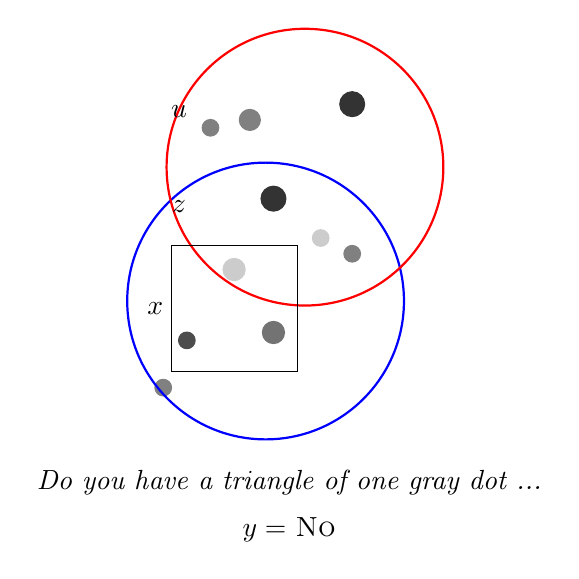
\begin{tikzpicture}

%\filldraw[gray!40] (0,0) circle (.3em);
%\filldraw[gray!100] (.25,0) circle (.38em);
%\filldraw[gray!160] (.5,0) circle (.45em);

\filldraw[gray!160] (-.2,.6) circle (.45em); % 76
\filldraw[gray!40] (-.7,-.3) circle (.4em); % 51
\filldraw[gray!40] (.4,.1) circle (.3em); % 52
\filldraw[gray!100] (.8,-.1) circle (.3em); % 66

% left
\filldraw[gray!140] (-1.3,-1.2) circle (.3em); % 13
\filldraw[gray!100] (-1.6,-1.8) circle (.3em); % 14
\filldraw[gray!110] (-.2,-1.1) circle (.4em); % 74

% right
\filldraw[gray!100] (-1,1.5) circle (.3em); % 28
\filldraw[gray!100] (-.5,1.6) circle (.38em); % 69
\filldraw[gray!160] (.8,1.8) circle (.45em); % 26

% agent plans 76
% \node[
%     draw,circle,dashed,blue,thick, minimum size=1.2em,
%     %label= left:$x$
% ] (x) at (-.2,.6) {};
% % m label
% % \filldraw[gray!40] (.4,.5) circle (.3em); % 52
% \node[
%     draw,circle,dashed,red,thick, minimum size=.6em,
%     %label=left:$m$
% ] (m) at (.4,.1) {};

\draw[blue,thick] (-.3,-.7) circle (5em);
\draw[red,thick] (.2,1) circle (5em);

% s label
\draw[draw=black] (-1.5,-1.6) rectangle (0.1,0);
%\node (s) at (-.8,1) {$s$};

% u label
% \draw[draw=black] (-1.2,1.3) rectangle (1.1,2.1);
%\node (u) at (-1.05,1.95) {$u$};
\node (u) at (-1.4, 1.7) {$u$};
\node (s) at (-1.4,0.5) {$z$};
% z label
%\node (z) at (-2.7,1) {$z$};
% d label
\node (d) at (-2.7,-.7) {$\mcD$};
\node (x) at (-1.7,-0.8) {$x$};
 
% \node (xe) at (-3.23,-3) {$x=$};
%\filldraw[gray!40] (-2.5,-3) circle (.3em); % 52
% \filldraw[gray!160] (-2.5,-3) circle (.45em); % 76
% \draw[dashed,blue,thick] (-2.5,-3) circle (.6em);

\node (v) at (-0, -3) {\textit{Do you have a triangle of one  gray dot ... }};

\node (y) at (-0,-3.6) {$y=$ \textsc{No}};
% \node (m) at (0,-3.6) {$m=$};
% \filldraw[gray!40] (.7,-3.6) circle (.3em); % 52
% \draw[dashed,red,thick] (.7,-3.6) circle (.5em);

%\node (v) at (-0, -4.2) {$y=$ No, I don't see those.};

\end{tikzpicture}
}
\caption{In \textsc{OneCommon},
the agent's perspective $\mcD$ is represented by the large blue circle,
and the partner's unobserved perspective by the red.
The shared dots $z$ are in both perspectives,
while the unshared dots $u$ are only in the red circle. 
The agent plan $x$ is given by the dots in the box,
and also described in language.
The partner response $y$ is a binary confirmation.
}
\label{fig:xzy}
\end{figure}

\subsection{Partner model}

% There are two challenges for planning with a partner model in \textsc{OneCommon}.
% First, marginalizing over the unobserved partner perspective, $\int_z p(y,z\mid x)dz$, is intractable because the dots in $z$ have continuous-valued sizes, colors, and positions.
% % This is solved by discretization.
% We address this using feature discretization.
% Second, the number of possible discretized partner perspectives $z$ is still large.
% We make marginalization tractable by decomposing the partner perspective $z$ into wo components: dots which are shared and unshared with the agent, %dots which are shared and unshared with the agent,
% and constrain the partner model to reason about them separately.
% breaking down the computation of marginalization into tractable steps.

We build a partner model by factoring the shared perspective $z$ and partner response $y$ as illustrated in Figure \ref{fig:xzy}. 
Formally,
\begin{align*}
p(y \mid x) &= \sum_z p(y\mid x,z)p(z) \\
&= \sum_{z,u}  p(y \mid x, z, u)p(z)p(u),
\end{align*}
where we introduce the latent variable $u$ representing the unshared dots in the partner perspective.

The shared dot prior, $p(z)$, is a distribution over subsets of $\mcD$, indicating which dots in the agent perspective $\mcD$ are shared with the partner.
The model $p(z)$ is initially uniform over dot subsets at the start of a game,
but is updated given evidence from the partner response $y$ at the end of each turn, $p(z \mid x, y)$. For notational simplicity we focus on the first turn.

The unshared dot prior, $p(u)$, is a distribution over the remaining partner dots.
Since the dots in $u$ are unobserved by the agent, we parameterize $p(u \mid s)$ using a uniform distribution over discretized features for each dot.
We ignore spatial features for dots in $u$
and discretize the other originally continuous features: size and color.%
\footnote{
We discretize size and color uniformly into 3 buckets based on their absolute range
across \textsc{OneCommon}.
}


%\justin{optional ->}
%The support of $p(u \mid s)$ is larger than $p(s)$: for $|u| = 3$, there are $9^3 = 728$ feature combinations.

%\justin{optional ->}
% The size of the support of $p(z)$ increases multiplicatively with the size of $p(u \mid s)$, making marginalization computationally costly.
% \daniel{insert forward reference here to where you describe how you address this?}

%\noindent \textbf{Response}
% The response model,
% % $$p(y \mid x,z) = p(c \mid x,z)p(m\mid z)p(w\mid c,m),$$
% factors into unshared, confirmation, and word models.
The confirmation model, $p(y \mid x,z)$, checks whether a partner will confirm or deny the agent plan. The partner confirms if they are able to resolve the plan $x$ to their perspective. Given a fully observed $z$ and $u$, resolution of a plan $x$ is performed by matching the features of $x$ to $z$ and $u$.
There are no trained parameters in resolution, as it depends only on the features of dots in $x$, $z$, and $u$.
See Appendix \ref{sec:feature-resolution} for the details of feature-based resolution.

In order to avoid jointly enumerating $z$ and $u$, the model reasons separately about $z$ and $u$ by making the simplifying assumption that plans are fully in $z$ or $u$.
This means that the model will deny if part of $x$ is in $z$, while the remainder is in $u$ (and $x$ is not fully contained in either $z$ or $u$):
\begin{align*}
p(y=\textsc{no}\mid x) &=\sum_{z,u} p(y=\textsc{no} \mid x, z, u)p(z,u)\\
&=\sum_z p(y=\textsc{no}\mid x, z )p(z)\\
&\quad \cdot \sum_u p(y=\textsc{no}\mid  x, u )p(u).
\end{align*}
Given the unsuccessful resolution of $x$ to both $z$ and $u$, the partner denies accurately with probability $\theta$, a hyperparameter.

% The confirmation model, $p(c \mid x,z,u)$, 
% checks if the partner confirms our plan
% based on their perspective.
% We make the simplifying assumption that a confirmation,
% $c = \text{\textsc{yes}}$, indicates that a plan $x$ resolves fully to either \justin{does either imply exclusive? its not an exclusive or} $z$ or $u$.\footnote{We ignore overlaps for computational efficiency, see Appendix \ref{sec:marginal-confirmation}}.
% % This means that the partner disconfirms if part of $x$ resolves to $s$ and the remainder to $u$,
% % and there is no other way to resolve $x$ to either $s$ or $u$.
% % We demonstrate how this assumption improves the computational complexity of computing the marginal confirmation distribution
% % in Appendix \ref{sec:marginal-confirmation}.
% When considering matches to $z$ all bucketed features (size, color, and spatial position) are checked.\footnote{
% The pairwise spatial position between dots  is bucketed into four
% relations: 
% above-left, above-right, below-left, or below-right.
% }
% When considering possible matches to $u$, spatial features are ignored for efficiency.

%\noindent \textbf{Response}
%Given a successful resolution of $x$ the partner confirms with probability $\theta$.
% The same parameter $\theta$ also determines disconfirmation given unsuccessful resolution.
% \daniel{how is $\theta$ set?}


% The mention model, $p(m \mid z)$, is a distribution over
% possible partner referents, represented as subsets of $z$.
% We assume that partner referents are not split between $s$ and $u$:
% mentions $m$ are chosen by first choosing either $s$ or $u$ with equal probability, then uniformly choosing a subset of dots from either $s$ or $u$ respectively.
% % allows same distributive trick

%The utterance model, $p(y \mid c)$, is a uniform distribution over sentences that confirm or deny the plan. \srush{This part needs to actually be written.}

\subsection{Inference}
\label{sec:inference}

% In the remainder of this section, we give the specifics of inference in \textsc{OneCommon}.
% As the goal of \textsc{OneCommon} is to find a dot in common,
% The agent plans by optimizing 
% Throughout, the agent marginalizes over the uniform $p(u\mid s)$,
% a conservative assumption that all unshared dots configurations are possible.
% This causes the agent to avoid plans that are likely to be incorrectly resolved to the unshared dots regardless of any information gathered,
% resulting in richer, more specific plans.
%\daniel{Justify this better, e.g. move the text from  "Belief update" (``avoid plans... any information gathered'') here. Or, might be worth adding something to reinforce that beliefs do still update in a useful way if possible, as otherwise this may seem like a big limitation. This doesn't have to come at this point in the paper, but it could help generally to have e.g. a qualitative example showing how the belief over the observed dots changes as we get more utterances.}

During inference, we need to compute $p(y \mid x)$ for all plans $x$,
which can be done in two steps: First, we marginalize over the unshared dots $u$.
This marginalization can be expressed in closed form.
For the details, see Appendix \ref{sec:unshared-marginal}.
Second, we marginalize over the possible set of shared dots $z$.
The computational cost of marginalization is the size of the power set of $\mcD$, $O(2^{|\mcD|})$.

%\footnote{Marginalization over the unshared perspective in the partner model can be precomputed for an entire dialogue given the agent perspective $\mcD$, thanks to the specifics of the partner model parameterization. See Appendix \ref{sec:information-gain} for the details on precomputing marginal distributions for planning.}

We utilize this distribution to compute the posterior on the shared perspective $z$, after observing a partner response to a plan,
$$ p(z \mid x,y) = \frac{ p(z, y \mid x)}{p(y \mid x)}.$$
This posterior then allows us to perform optimization over plans with respect to the expected information gain, as well as update our beliefs given the partner response.

% Accounting for the unshared dots in the partner perspective in this manner encourages the agent to choose plans which are less likely to have counterparts that only the partner can see.

\noindent \textbf{Planning} Planning optimizes the expected information gain with respect to the shared perspective $z$:
$$\argmin_x \Es{y\mid x}{H(z \mid x,y)}.$$
Computing $p(y \mid x)$ has cost $O(2^{|\mcD|})$,
while there are also $O(2^{|\mcD|})$ plans.\footnote{
Plans $x$ are subsets of $\mcD$ that the agent would like to ask the partner about.
}
As a result, optimizing this objective takes $O(2^{2|\mcD|})$ computation, and is performed in less than one second on CPU.% in real-time.
% \daniel{might be a good place to say that this is still fast enough to run on a CPU in real-time, or give a forward ref to where you say that}

\textbf{Belief update}
The belief update directly uses the posterior distribution $p(z \mid x,y)$, as described in Section \ref{sec:planning}.

During gameplay in \textsc{OneCommon}, the agent either directly observes the symbolic response $y$ or receives a description of $y$ in natural language.
In order to process the natural language dialogue,
we use a classifier to extract $y$ from natural language. 
Additionally, the partner can mention dots of their own, either symbolically or described in text.
The agent incorporates partner mentions into its belief by treating them as a confirmed plan.
We use another classifier to extract partner mentions from text.
We give the details of both the response and mention classifiers in Section \ref{sec:exp}.

\textbf{Selection}
To determine when to select a dot, the agent uses a threshold on the entropy $H[z]$, given by the hyperparameter $\tau$.
The agent them communicates which dot to select by
describing the configuration of four dots with the
highest marginal probability of being shared,
as well as the dot within that configuration that is most likely to be shared.
The agent then selects the described dot.


\section{Feature-based resolution}
\label{sec:feature-resolution}
Feature-based resolution featurizes a plan $x$
then compares the features to all subsets of dots
in the partner domain $\mcD$.
The set of features used for each plan $x$ is given by the shape and size
each dot in the plan, bucketed into 3 bins based on the range of each feature.
The pairwise positions, limited to above-left, above-right, below-left, and below-right, are also contained in the feature set.
We provide an example of feature-based resolution in Figure
\ref{fig:resolution-example}.

Given a plan $x$, feature-based resolution
must compare all the features of the plan,
of which there are $O(|x|^2)$,
to all partial permutations of subsets size $|x|$ taken from $\mcD$,
of which there are $O(|\mcD|^{|x|})$.
This can be precomputed at the start of a dialogue.

When resolving $x$ to unshared dots, we ignore spatial features.

\begin{figure}[t]
\setlength{\abovecaptionskip}{0pt}

\centering

\scalebox{1.1}{
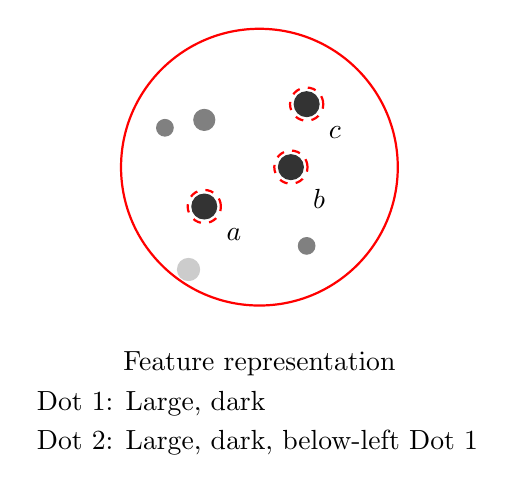
\begin{tikzpicture}


\filldraw[gray!160] (-.5,.5) circle (.45em); % 76
\filldraw[gray!40] (-.7,-.3) circle (.4em); % 51
\filldraw[gray!100] (.8,0) circle (.3em); % 66
\filldraw[gray!100] (-1,1.5) circle (.3em); % 28
\filldraw[gray!100] (-.5,1.6) circle (.38em); % 69
\filldraw[gray!160] (.8,1.8) circle (.45em); % 26
\filldraw[gray!160] (.6,1) circle (.45em); % 26

%\draw[dashed,blue,thick] (-.3,-.7) circle (5em);
\draw[red,thick] (.2,1) circle (5em);

\node[
    draw,circle,dashed,red,thick, minimum size=1.2em,
    label=below right:$a$
] (a) at (-.5,.5) {};
\node[
    draw,circle,dashed,red,thick, minimum size=1.2em,
    label=below right:$c$
] (c) at (.8,1.8) {};
\node[
    draw,circle,dashed,red,thick, minimum size=1.2em,
    label=below right:$b$
] (b) at (.6,1) {};

\node (f) at (.2, -1.5) {Feature representation};

\node[anchor=west] (f1) at (-2.75, -2) {Dot 1: Large, dark};
\node[anchor=west] (f2) at (-2.75, -2.5) {Dot 2: Large, dark, below-left Dot 1};

\end{tikzpicture}
}
\vspace{1em}
\caption{
An example of feature-based resolution.
The above feature representation for a pair of dots
resolves to dot configurations $\set{(a,b), (a,c), (b,c)}$.
}
\label{fig:resolution-example}
\end{figure}

\section{Resolution to unshared dots}
\label{sec:unshared-marginal}
The partner model, with the assumption that
$x$ cannot be split between $z$ and $u$,
is given by
\begin{align*}
&p(y=\textsc{no} \mid x)\\
&= \sum_{z,u}p(y = \textsc{no} \mid x,z,u)p(z)p(u)\\
&\approx \sum_{z,u}p(y=\textsc{no} \mid x,z)p(z) p(y=\textsc{no} \mid  x,u)p(u)\\
&= \sum_z p(y=\textsc{no} \mid x,z)p(z) \sum_u p(y=\textsc{no} \mid  x,u)p(u)\\
&= \sum_z p(y=\textsc{no} \mid x,z)p(z) \sum_u p(y=\textsc{no},u \mid  x).
\end{align*}
The probability a plan $x$ resolves to the unshared dots $u$ is
\begin{align*}
\sum_u p(y=\textsc{no},u \mid x)
&= 1-\theta {|u|\choose|x|}\frac{B^{2 \cdot (|u|-|x|)}}{B^{2\cdot|x|}},
\end{align*}
where $B$ is the feature bucket size,
given $|u| \ge |x|$.
This relies on the assumption that spatial features are ignored when resolving to unshared dots.

\section{Planning objective}
In addition to maximizing the information gain,
we also add an entropy rate constraint to the planning objective,
motivated by the entropy rate constancy and uniform information density hypotheses \citep{erc,uid,ercdial}.

In order to enforce a limit on the entropy rate, 
we limit the surprisal of the next mention proposals
under a mention model $p(x_t | x_1,\ldots,x_{t-1})$ \justin{how to include partner mentions and confirmations?}.
We could utilize the belief state $p(z = x_t)$ for this model \justin{include other history?}; however, this model is not sensitive to the ordering of plans in $h$.
We model mentions with an linearly decaying cache model,
\citep{cache}:
\begin{align*}
&p_{\text{cache}}(x_T \mid h)\\
&\propto \prod_d e^{\beta m([x_T]_d,h)
    \mathbf{1}([x_T]_d\in h)
}
e^{\alpha\mathbf{1}([x_T]_d \notin h)},
\end{align*}
where
$$m([x_T]_d,h) = T - \argmax_t t\mathbf1([x_T]_d \in h_t),$$
and $\beta$ and $\alpha$ are hyperparameters that control
the cost of unmentioned dots and recency bias respectively.

We also experiment with a supervised neural model \justin{include other history?}.

\section{Partner confusion model}
In the previous section, we introduced processing cost (as a channel capacity constraint) in the planning objective to limit the amount of information conveyed by an agent.
This is an anti-causal approach: Adding processing cost to the objective does not model the effects of a plan.
In this section we give a causal model of partner confusion as a result of processing cost.

The generative process for a response, given in Section \ref{sec:plan-oc}, is given by:
given a plan $x$, resolve that plan to the shared dots $z$ or unshared dots $u$. If the plan resolves to one or both, the partner gives a confirmation $y = \textsc{Yes}$.
Unfortunately, this partner model assumes superhuman levels of resolution.

In our human studies, we found that certain plans are difficult for humans to resolve. Plans that involve contextually vague color or size descriptors, or dots that are too far apart result in the denial of a plan that should have been confirmed.
Additionally, we believe some human players were frustrated by the information-dense descriptions of inhuman model plans, leading to poor success rates.
In this section we describe several changes to the partner model that better reflect the behaviour of a human partner.

There are three desiderata:
\begin{enumerate}
\item Spatial locality: The partner will deny a plan if the dots are too far apart
\item Channel capacity: The partner will deny a plan if there is too much new information
\item Information locality: The partner has limited memory and will treat repeated old information as new information
\end{enumerate}

We incorporate these desiderata by building them into the partner model.
We utilize a product of experts formulation,
where we combine the original partner resolution model
with a confusion model.
The goal of the confusion model is to model the effort a human partner would be willing to put into resolving a plan.
The product of experts formulation allows the confusion model to
vote against confirmation,
resulting in the response model predicting denial if the plan is theoretically resolvable, but too confusing for a human to actually understand.

Let $h$ be the history of all previous plans,
with $[h]_t = x_t$.
The full partner response model is given by
$$
p(y \mid x, z, u, h)
\propto \underbrace{p_r(y \mid x,z,u)}_{\text{resolution}}
\underbrace{p_c(y \mid x,z,h)}_{\text{confusion}}.
$$
The confusion model itself is a product of experts,
consisting of spatial and temporal confusion models:
$$
p_c(y\mid x,z,h) \propto
\underbrace{p(y \mid x,z)}_{\text{spatial}}
\underbrace{p(y \mid x,h)}_{\text{temporal}}.
$$

\subsection{Spatial model}
For the spatial model, we assume a plan is more likely to be denied if the dots in the plan are far apart.
A first approach would be to either use the distance between the furthest pair of dots, the sum of the pairwise distances between dots, or the area of the convex hull of the dots.
However, as the distances of dots may vary,
we instead use the relative rankings of dot distances.
This mimics one possible method of dot resolution, where the partner first finds an anchor dot then searches nearby to find the remaining dots in the plan.
As a result, we have
$$
p(y = \textsc{No} \mid x)
= \min_{d\in x} \frac{
\sum_{d'\in x} r(d,d')
}{
1+\sum_{i=7-|x|+1}^7 i
},
$$
where $r(d,d')$ gives the rank of dot $d'$ to $d$ in order of increasing distance given the agent's perspective.
%\justin{will fix up later}
nswer both time, and take that into account with the partner model.

\section{Supervised partner model}


\section{Selection objective}

\section{Describing plans}
The success of an agent that plans through a partner model is limited
by the accuracy of its partner model.
While the partner model predicts the partner's reaction to the agent's plan,
a human partner receives a natural language description of the agent's plan.
For the partner model to be accurate, the plan description must be precise.

Preliminary experiments indicate that a model from previous work \citep{fried}
loses precision when describing plans involving more than a single dot.
We hypothesize that this is due to data imbalance.



\end{document}

